\documentclass[conference]{IEEEtran}
\usepackage{amsmath}
\usepackage{amssymb}
\usepackage{array}
\usepackage{booktabs}
\usepackage{color}
\usepackage{float}
\usepackage{graphicx}
\usepackage{ifpdf}
\usepackage[utf8]{inputenc}
\usepackage{keyval}
\usepackage{listings}
\usepackage{moresize}
\usepackage{multirow}
\usepackage[numbers,sort&compress,square]{natbib}
\usepackage{paralist}
\usepackage{rotating}
\usepackage{soul}
% \usepackage[style=base]{subcaption}
\usepackage{srcltx}
\usepackage{url}
\usepackage[dvipsnames]{xcolor}
\usepackage{xspace}
\usepackage{wrapfig}
\usepackage{hyperref}
% \usepackage{caption}
\usepackage{enumitem}

\definecolor{listinggray}{gray}{0.95}
\definecolor{darkgray}{gray}{0.7}
\definecolor{commentgreen}{rgb}{0, 0.4, 0}
\definecolor{darkblue}{rgb}{0, 0, 0.6}
\definecolor{purple}{rgb}{0.6, 0, 0.6}
\definecolor{middleblue}{rgb}{0, 0, 0.75}
\definecolor{darkred}{rgb}{0.4, 0, 0}
\definecolor{brown}{rgb}{0.5, 0.5, 0}
\definecolor{dkgreen}{rgb}{0,0.5,0}
\definecolor{orange}{rgb}{1,.5,0}
\definecolor{dandelion}{cmyk}{0,0.29,0.84,0}

\lstset{ 
  backgroundcolor=\color{white},   % choose the background color; you must add \usepackage{color} or \usepackage{xcolor}; should come as last argument
  basicstyle=\ttfamily\footnotesize,        % the size of the fonts that are used for the code
  breakatwhitespace=false,         % sets if automatic breaks should only happen at whitespace
  breaklines=true,                 % sets automatic line breaking
  captionpos=b,                    % sets the caption-position to bottom
  commentstyle=\color{purple},    % comment style
  deletekeywords={...},            % if you want to delete keywords from the given language
  escapeinside={\%*}{*)},          % if you want to add LaTeX within your code
  extendedchars=true,              % lets you use non-ASCII characters; for 8-bits encodings only, does not work with UTF-8
  % frame=single,                    % adds a frame around the code
  keepspaces=true,                 % keeps spaces in text, useful for keeping indentation of code (possibly needs columns=flexible)
  keywordstyle=\color{orange},       % keyword style
  language=python,                 % the language of the code
  morekeywords={*,...},            % if you want to add more keywords to the set
  numbers=left,                    % where to put the line-numbers; possible values are (none, left, right)
  numbersep=5pt,                   % how far the line-numbers are from the code
  numberstyle=\tiny\color{darkgray}, % the style that is used for the line-numbers
  rulecolor=\color{black},         % if not set, the frame-color may be changed on line-breaks within not-black text (e.g. comments (green here))
  showspaces=false,                % show spaces everywhere adding particular underscores; it overrides 'showstringspaces'
  showstringspaces=false,          % underline spaces within strings only
  showtabs=false,                  % show tabs within strings adding particular underscores
  stepnumber=2,                    % the step between two line-numbers. If it's 1, each line will be numbered
  stringstyle=\color{commentgreen},     % string literal style
  tabsize=2,                       % sets default tabsize to 2 spaces
  % title=\lstname                   % show the filename of files included with \lstinputlisting; also try caption instead of title
}

\usepackage[normalem]{ulem}
\makeatletter
\def\cyanuwave{\bgroup \markoverwith{\lower3.5\p@\hbox{\sixly \textcolor{cyan}{\char58}}}\ULon}
\def\reduwave{\bgroup \markoverwith{\lower3.5\p@\hbox{\sixly \textcolor{red}{\char58}}}\ULon}
\def\blueuwave{\bgroup \markoverwith{\lower3.5\p@\hbox{\sixly \textcolor{blue}{\char58}}}\ULon}
\font\sixly=lasy6 % does not re-load if already loaded, so no memory problem.
\makeatother

\usepackage{pgfplots}
\pgfplotsset{compat=newest}
\usepgfplotslibrary{fillbetween}
\usetikzlibrary{patterns}

\usepackage{siunitx}
\DeclareSIUnit{\calorie}{cal}
\usepackage[outline]{contour}

\usepackage{makecell}

%\usepackage{xcolor}

\newif\ifdraft
\drafttrue
\ifdraft
 \newcommand{\N}[1]{\textbf{*** NOTE: #1}\xspace}
 \newcommand{\jhanote}[1]{ {\textcolor{red} { ***SJ: #1 }}}
 \newcommand{\mtnote}[1]{ {\textcolor{orange} { ***MT: #1 }}}
 \newcommand{\note}[1]{ {\textcolor{brown} { *** #1 }}}
 \newcommand{\jdnote}[1]{ {\textcolor{cyan} { ***JD: #1 }}}
 \newcommand{\dwwnote}[1]{ {\textcolor{blue} { ***DWW: #1 }}}
\else
 \newcommand{\N}[1]{}
 \newcommand{\jhanote}[1]{}
 \newcommand{\mtnote}[1]{}
 \newcommand{\jdnote}[1]{}
 \newcommand{\dwwnote}[1]{}
 \newcommand{\note}[1]{}
\fi

\newcommand{\cloud}{cloud\xspace}
\newcommand{\clouds}{clouds\xspace}
\newcommand{\pilot}{Pilot\xspace}
\newcommand{\pilots}{Pilots\xspace}
\newcommand{\pilotjob}{Pilot-Job\xspace}
\newcommand{\pilotjobs}{Pilot-Jobs\xspace}
\newcommand{\pilotcompute}{Pilot-Compute\xspace}
\newcommand{\pilotcomputedescription}{Pilot-Compute Description\xspace}
\newcommand{\pilotdescription}{Pilot-Description\xspace}
\newcommand{\pilotcomputes}{Pilot-Computes\xspace}
\newcommand{\pilotdata}{Pilot-Data\xspace}
\newcommand{\pilotdatadescription}{Pilot-Data Description\xspace}
\newcommand{\pilotdataservice}{Pilot-Data Service\xspace}
\newcommand{\pilotcomputeservice}{Pilot-Compute Service\xspace}
\newcommand{\computedataservice}{Compute-Data Service\xspace}
\newcommand{\computeunitdescription}{Compute-Unit Description\xspace}
\newcommand{\dataunitdescription}{Data-Unit Description\xspace}
\newcommand{\pilotmapreduce}{PilotMapReduce\xspace}
\newcommand{\mrmg}{MR-Manager\xspace}
\newcommand{\pstar}{P*\xspace}
\newcommand{\pd}{PD\xspace}
\newcommand{\pc}{PC\xspace}
\newcommand{\pcs}{PCs\xspace}
\newcommand{\pj}{PJ\xspace}
\newcommand{\pjs}{PJs\xspace}
\newcommand{\pds}{Pilot Data Service\xspace}
\newcommand{\computeunit}{Compute-Unit\xspace}
\newcommand{\computeunits}{Compute-Units\xspace}
\newcommand{\dataunit}{Data-Unit\xspace}
\newcommand{\dataunits}{Data-Units\xspace}
\newcommand{\du}{DU\xspace}
\newcommand{\dus}{DUs\xspace}
\newcommand{\dud}{DUD\xspace}
\newcommand{\cu}{CU\xspace}
\newcommand{\cus}{CUs\xspace}
\newcommand{\cud}{CUD\xspace}
\newcommand{\su}{SU\xspace}
\newcommand{\sus}{SUs\xspace}
\newcommand{\schedulableunit}{Schedulable Unit\xspace}
\newcommand{\schedulableunits}{Schedulable Units\xspace}
\newcommand{\cc}{c\&c\xspace}
\newcommand{\CC}{C\&C\xspace}
\newcommand{\up}{\vspace*{-1em}}
\newcommand{\upp}{\vspace*{-0.5em}}
\newcommand{\numrep}{8 }
\newcommand{\samplenum}{4 }
\newcommand{\tmax}{$T_{max}$ }
\newcommand{\tc}{$T_{C}$ }
\newcommand{\tcnsp}{$T_{C}$}
\newcommand{\bj}{BigJob\xspace}
\newcommand{\irods}{iRODS\xspace}

\newcommand{\I}[1]{\textit{#1}\xspace}
\newcommand{\B}[1]{\textbf{#1}\xspace}
\newcommand{\T}[1]{\texttt{#1}\xspace}
%\newcommand{\C}[1]{\textsc{#1}\xspace}

\newcommand{\mr}[1]{\multirow{2}{*}{#1}}%
\newcommand{\mc}[2]{\multicolumn{#1}{l}{#2}}

\lstdefinestyle{myListing}{
  frame=single,
  backgroundcolor=\color{listinggray},
  %float=t,
  language=C,
  basicstyle=\ttfamily \footnotesize,
  breakautoindent=true,
  breaklines=true
  tabsize=2,
  captionpos=b,
  aboveskip=0em,
  belowskip=-2em,
  %numbers=left,
  %numberstyle=\tiny
}

\lstdefinestyle{myPythonListing}{
  frame=single,
  backgroundcolor=\color{listinggray},
  %float=t,
  language=Python,
  basicstyle=\ttfamily \scriptsize,
  breakautoindent=true,
  breaklines=true
  tabsize=2,
  captionpos=b,
  %numbers=left,
  %numberstyle=\tiny
}



%  \setlength{\parskip}{0.05ex} % 1ex plus 0.5ex minus 0.2ex}
%  \setlength{\parsep}{0pt}
%  %\setlength{\headsep}{0pt}
%  \setlength{\topskip}{0pt}
%  \setlength{\topmargin}{0pt}
%  %\setlength{\topsep}{0pt}
%  \setlength{\partopsep}{0pt}

% This is now the recommended way for checking for PDFLaTeX:


\ifpdf
\DeclareGraphicsExtensions{.pdf, .jpg, .tif}
\else
\DeclareGraphicsExtensions{.ps,  .eps, .jpg}
\fi

\tolerance=1000
\hyphenpenalty=10


\begin{document}


% \title{Alchemical and Endpoint Free Energy Calculations at Scale}

%\title{Rapid, Concurrent and Adaptive Extreme-scale Free energy calculation}

\title{Trading-off Accuracy with Computational Cost: Adaptive Algorithms to Reduce Time to Clinical Insight}



% \author{Jumana Dakka$^{1}$,  Kristof Farkas-Pall$^{3}$, David W. Wright$^{3}$, .... Shantenu Jha$^{1}$$^{,2}$, \\

\author{Jumana Dakka$^{*,1}$, Kristof Farkas-Pall$^{*,2}$, Vivek Balasubramanian$^{1}$ , Matteo Turilli$^{1}$, \\
 Shunzhou Wan$^{2}$, David W Wright$^{2}$, Stefan Zasada$^{2}$, \\\
 Peter V Coveney$^{2}$, Shantenu Jha$^{1,3}$ \\

  \small{\emph{$^{1}$ Rutgers, the State University of New Jersey, Piscataway, NJ 08854, USA}}\\
   \small{\emph{$^{2}$ University College London, London, UK, WC1H 0AJ}}\\
   \small{\emph{$^{3}$ Brookhaven National Laboratory, Upton, New York, 11973}}\\
   \small{\emph{$^{*}$ Contributed Equally}}
}


\date{}
\maketitle

\begin{abstract}


The efficacy of drug treatments depends on how tightly small molecules bind to
their target proteins. Quantifying the strength of these interactions (the so
called ‘binding affinity’) is a grand challenge of computational chemistry,
surmounting which could revolutionize drug design and provide the platform for
patient specific medicine. Recently, evidence from blind challenge predictions
and retrospective validation studies has suggested that molecular dynamics
(MD) can now achieve useful predictive accuracy (1 kcal/mol) 
This accuracy is sufficient to greatly accelerate lead optimization 

To translate these advances in predictive accuracy so as to impact clinical
and/or industrial decision making requires that binding free energy results
must be turned around in timescales of hours or days without loss of accuracy.
This requires advances in algorithms, scalable software systems, and
intelligent and efficient utilization of supercomputing resources.
Specifically, it requires refining algorithms and developing technologies to
marshal huge simulation campaigns.

This work is motivated by the real world problem of providing clinical insight
from drug candidate data on a time scale that is as short as possible.
Specifically, we reproduce results from a collaboration project between UCL
and GlaxoSmithKline to study a congeneric series of drug candidates binding to
the BRD4 protein -- inhibitors of which have shown promising preclinical
efficacy in pathologies ranging from cancer to inflammation. In this SCALE
challenge, we demonstrate the use of a framework -- HTBAC, designed to support
the aforementioned requirements of accurate and rapid drug binding affinity
calculations. HTBAC facilitates the execution of the numbers of simulations
while supporting the adaptive execution of algorithms. Furthermore, HTBAC
enables the selection of experimental parameters during runtime, which can in
principle optimize the use of computational resources whilst producing results
with a target uncertainty.

\end{abstract}

% \cite{shirts-mobley-chodera:2007:annu-rep-comput-chem:prime-time, 
% abel:jacs:2015:fep-plus}.
% \cite{shirts-mobley-brown:2009:sbdd}.


% ---------------------------------------------------------------------------
% Introduction
% ---------------------------------------------------------------------------
%\section{Introduction}\label{sec:intro}




% ---------------------------------------------------------------------------
% Scientific Motivation
% ---------------------------------------------------------------------------

\section{Scientific Motivation}\label{sec:motivation}

% This work is motivated by the real world problem of providing clinical insight
% from drug candidate data on a time scale that is as short as possible.
% Specifically, we reproduce results from a collaboration project between UCL
% and GlaxoSmithKline to study a congeneric series of drug candidates binding to
% the BRD4 protein (inhibitors of which have shown promising preclinical
% efficacy in pathologies ranging from cancer to
% inflammation)~\cite{Wan2017brd4}.


Bromodomain-containing proteins, and in particular the four members of the BET
(bromodomain and extra terminal domain) family, are currently a major focus of
research in the pharmaceutical industry. Small molecule inhibitors of these
proteins have shown promising preclinical efficacy in pathologies ranging from
cancer to inflammation. Indeed, several compounds are progressing through
early stage clinical trials and are showing exciting early
results~\cite{Theodoulou2016}. One of the most extensively studied targets in
this family is the first bromodomain of bromodomain-containing protein 4
(BRD4-BD1) for which extensive crystallographic and ligand binding data are
available~\cite{Bamborough2012}.

\begin{figure}
  \centering
  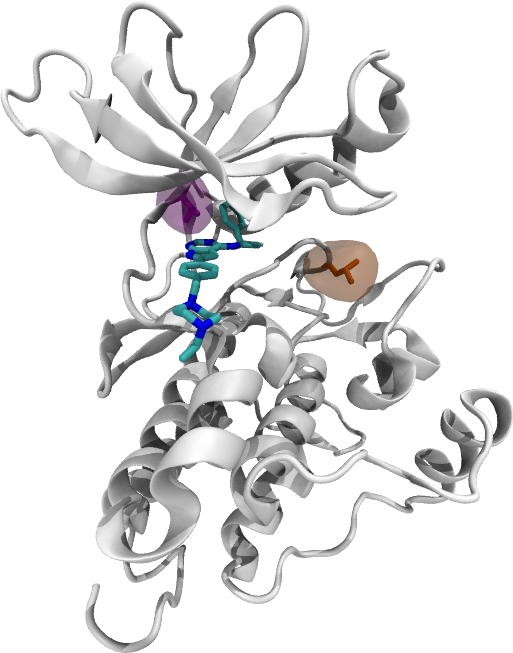
\includegraphics[width=0.60\columnwidth]{./egfr.png}
  \caption{Cartoon representation of the EGFR kinase bound to the inhibitor
  AEE788 shown in chemical representation (based on PDB:2J6M). Two residues
  implicated in modulating drug efficacy are highlights; in pink T790 and in
  orange L858. Mutations to either of these residues significantly alter the
  sensitivity to TKIs.}\label{fig:egfr}
\end{figure}


We have investigated a congeneric series of ligands binding to BRD4-BD1 (we shall
from now on refer to this are simply BRD4). This was performed in the context
of a blind test of the protocols in collaboration with
GlaxoSmithKline~\cite{Wan2017brd4}. The goal was to benchmark the ESMACS and
TIES protocols in a realistic drug discovery scenario. In the original study,
we investigated chemical structures of 16 ligands based on a single
tetrahydroquinoline (THQ) scaffold. These studies employed two different
algorithms (simulation protocols), known as TIES and ESMACS~\cite{Bhati2017},
both based on multiple simulations of the same system. Drug design projects
have limited resources, so initially large numbers of compounds must be
cheaply screened to eliminate poor binders (using ESMACS), before more
accurate methods (such as TIES) are needed as good binders are refined and
improved.

In order to support such investigations, in addition to scale, the protocols
must be executed to utilize  flexible resource management schemes where based
upon intermediate results at runtime, resources can be (re-)allocated between
instances of different protocols or systems, for example, when one calculation
has converged whilst another has not. Such adaptability makes it easier to
manage complex programs where efficient use of resources is required in order
to achieve a time to completion of studies comparable to those of high
throughput chemistry.

This work is motivated by the real world problem of providing clinical insight
from drug candidate data (study a congeneric series of drug candidates binding
to the BRD4 protein) on a time scale that is as short as possible. In this
SCALE challenge, we demonstrate the use of a framework -- HTBAC, designed to
support the aforementioned requirements of accurate and rapid drug binding
affinity calculations. HTBAC facilitates the execution of the numbers of
simulations while supporting the adaptive execution of algorithms.
Furthermore, HTBAC enables the selection of experimental parameters during
runtime, which can in principle optimize the use of computational resources
whilst producing results with a target uncertainty.

% We demonstrate the scalability and flexibility of HTBAC.

% In order to support such investigations, in addition to being scalable, HTBAC
% must be enhanced to support flexible resource reallocations schemes where
% resources can be moved between simulations run using different protocols or
% systems, for example, when one calculation has converged whilst another has
% not. This adaptability makes it easier to manage complex programmes where
% efficient use of resources is required in order to achieve a time to
% completion of studies comparable to those of high throughput chemistry.




% Here we focus on the first seven of these ligands to test and refine the
% protocols used and the way in which they were executed. The results of our
% previous work provide a benchmark of both accuracy and statistical uncertainty
% to which we can compare our new results.
 
\section{Methods and Models}

In this section we outline the computational methods employed and the physical
system (drug candidates) studied. We discuss how computational methods have
been co-designed with the software systems to support scalable approaches on
the largest supercomputers.

\subsection{Binding Affinity Calculation Protocols}\label{sec:bac}

Computing accurate protein-drug binding affinities (also known as binding free
energies) requires a simulation technique which captures the chemical detail
of the system. MD simulations are the time dependent numerical integration of
the classical equations of motion for molecular systems. Application of MD to
atomistic models of proteins and their ligands can be used to answer questions
about the properties of a specific system often more readily than experiments
on the actual system. Free-energy calculations in the framework of MD
simulations not only yield quantitative estimates of binding strength but also
provide insights into the most important interactions driving the process.
Evidence from blind challenge predictions and retrospective validation studies
has suggested that molecular dynamics (MD) can now achieve useful predictive
accuracy (1 kcal/mol) 
\cite{shirts-mobley-chodera:2007:annu-rep-comput-chem:prime-time, abel:jacs:2015:fep-plus}. This accuracy is sufficient to greatly
accelerate lead optimization \cite{shirts-mobley-brown:2009:sbdd}.

Statistical mechanics provides the prescription for calculating such
macroscopic quantities as ensemble averages of microscopic states.
Traditionally, these macroscopic properties have usually been calculated from
the time average of a single “long” duration trajectory. An intuitive and
potentially more time efficient method to capture the mixing dynamics required
to describe an equilibrium thermodynamic state is the use of an ensemble of
separate trajectories. \cite{Coveney2016}

The major sources of error in free energy calculations are the representation
of the system chemistry encoded in the forcefield used, finite sampling and
the free energy estimator. Protocols developed in the Coveney labs have
obtained accurate and precise results which successfully reproduce
experimental binding free energies from a wide range of systems.
\cite{Wright2014, Wan2017brd4, Wan2015, Wan2011} Comparisons of results
obtained for a large set of sequences will provide valuable insights on the
importance of choices made in simulation and analysis for the overall accuracy
and predictive power of free energy calculations, and facilitate the
refinement of our protocols.


Most methods for calculating binding affinities fit into one of two broad classes; so called alchemical and endpoint methodologies. 
Alchemical free energy calculations employ unphysical (“alchemical”) intermediates to calculate changes in free energies between two systems. 
It is common in these methods to refer to a variable, $\lambda$, which describes the path taken to transform one protein sequence (or ligand) into another. 
Endpoint methods, as the name suggests, consider the difference in energy between bound and unbound structures. 
To obtain information on the differences in binding affinity of different sequences for a panel of kinase inhibitors requires a deployment of various strategies, incorporating both alchemical and endpoint approaches. 
In this work we deploy approaches from both of these classes.


\subsubsection{Alchemical Protocol (TIES)}\label{sec:ties}

Alchemical methods employ MD simulations of unphysical, alchemical intermediate states that attenuate the interactions of the small molecule with its environment. 
These alchemical intermediate states include both the fully-interacting complex as well as replicas in which the ligand does not interact with its environment, and allow the total free energy of binding—including entropic and enthalpic contributions—to be efficiently computed. Typically, the alchemical path between the states of interest is described by a parameter, $\lambda$, which varies between 0 for the initial and 1 for the final state of the transformation of interest. 
Sampling is then performed at a series of points along this path and the gradient of the energy integrated to calculate the binding affinity.
Simulations conducted at a given $\lambda$ value are said to be sampling a $\lambda$ window at that point.

The TIES (thermodynamic integration with enhanced sampling) protocol, developed within the Coveney lab, employs ensemble sampling at each $\lambda$ window to yield reproducible, accurate, and precise relative binding affinities. 
\cite{ Wan2017brd4} Based on the direct calculation of ensemble averages, it allows us to determine statistically meaningful results along with complete control of errors. 
As currently designed, TIES computes the change in binding affinity between two related system (termed ‘relative binding affinities’).


\subsubsection{Endpoint Protocol (ESMACS)}\label{sec:esmacs}

Computationally cheaper, but less rigorous methods, endpoint methods have been used to directly compute the binding strength of a drug to the target protein from MD simulations (as opposed to differences in affinity). 

We have developed an ensemble-based endpoint protocol called ESMACS (enhanced sampling of molecular dynamics with approximation of continuum solvent). The protocol is built on the popular molecular mechanics Poisson–Boltzmann surface area (MMPBSA) \cite{Massova1999} method which makes a continuum approximation for the aqueous solvent in order to obtain results on practical timescales. Commonly, MMPBSA analyses are performed on a single MD trajectory, or even a single structure. We have demonstrated the lack of reproducibility of such an approach in both HIV-1 protease and MHC systems, with calculations for the same protein-ligand combination, with identical initial structure and force field, shown to produce binding affinities varying by up to 12 kcal/mol for small ligands (flexible ligands can vary even more). \cite{Wan2015} ESMACS employs MMPBSA to produce ensemble- based, converged and reproducible, determinations of binding free energies (separate ligand and receptor trajectories can also be used to account for adaptation energies). This provides a rapid quantitative approach sensitive enough to determine changes in binding free energies which differentiate susceptible and resistant sequences (typically of the order of 2 kcal/mol).



% ---------------------------------------------------------------------------
% Section II
% ---------------------------------------------------------------------------
\subsection{BRD4 System}\label{sec:system_description}

Initial coordinates for the protein-ligand system were taken from the X-ray
crystal structure PDB ID: 4BJX.
% ~\cite{Wyce2013}. 
This structure contains a
ligand based on the THQ template and other ligands were alligned with this
common scaffold. Preparation and setup of the simulations were implemented
using our automated tool, BAC~\cite{Sadiq2008}. This process including
parametrization of the compounds, solvation of the complexes, electrostatic
neutralization of the systems by adding counterions and generation of
configurations files for the simulations. The AMBER ff99SB-ILDN
% ~\cite{Lindorff-Larsen2010} 
force field was used for the protein, and TIP3P was used
for water molecules. Compound parameters were produced using the general AMBER
force field (GAFF)~\cite{Wang2004} with Gaussian 03
%~\cite{Frisch} 
to optimize compound geometries and to determine electrostatic potentials at
the Hartree–Fock level with 6-31G** basis functions. The restrained
electrostatic potential (RESP) module in the AMBER package
%~\cite{Case2005} 
was used to calculate the partial atomic charges for the compounds. All systems
were solvated in orthorhombic water boxes with a minimum extension from the
protein of 14 \AA\ (the resulting systems contain approximately 40 thousand
atoms).

% \subsection{Scientific Challenge}



% ---------------------------------------------------------------------------
% Section III
% ---------------------------------------------------------------------------
% \section{Performance Metrics}\label{sec:performance}

% % \subsection{Ensemble Molecular Dynamics}\label{sec:emd}

% TIES is rigorous but computationally expensive and has a limited range of
% applicability; ESMACS is approximate but can be employed across any set of
% ligands at lower computational cost. Both protocols are designed to simulate a
% large range of mutations. A single protocol instance represents a unique
% physical system. Each protocol instance contains a pipeline which maps to a
% sequence of simulations steps which include minimization, equilibration and
% production MD simulation. These simulation pipelines are replicated, where
% replicas differ only by their parameter configurations, namely initial
% velocities, which are randomly generated and assigned by the MD engine at the
% start of execution. ESMACS consists of 25 replicas i.e. 25 pipelines, while
% TIES consists of 13 $\lambda$ windows, which are additional sampling
% parameters, and 5 replicas for a total of 65 pipelines. The additional
% pipelines in TIES contribute to the greater computational cost. Both protocols
% run for a total of 6 ns simulation durations. ESMACS produces 3.5 GB/system
% (24 MB/ns) while TIES produces 10 GB/system (24 MB/ns). Each simulation step
% in TIES and ESMACS requires 32 cores. Protocols run approximately 10-12 hours,
% depending on the physical system and the number of timesteps provided by the
% user.

% \mtnote{We need a better description of TIES and ESMACS.}

% \mtnote{Is the title of the section wrong? I see no mention of performance
% metrics.}

% ---------------------------------------------------------------------------
% Section IV
% ---------------------------------------------------------------------------
\section{Computational Challenges}\label{sec:cc}

\jhanote{There is no mention of adaptivity as a challenge. Vivek should add
from his paper.}

\jhanote{Need better organization. Separate out challenge of (i) simple and
usable software systems, (ii) scale and interoperability, and (iii)
adaptivity challenges. }\mtnote{Better?}

As the nature of scientific inquiry and the applications to support that
inquiry evolve, there is a critical need to support the execution of
scientific workflows on high-performance computing (HPC) infrastructures.
This poses three main challenges: (1) scaling the distributed execution of
workflows; (2) developing simple and usable workflow systems for HPC
resources; and (3) implementing runtime adaptivity.

\subsection{Scalability}

Applications composed of multiple tasks with dependences that determine the
order of their execution are referred to as `workflows'. Often times, the
structure of the task dependencies is simple and adheres to discernible
patterns, even though the individual tasks and their duration are
non-trivially distinct. Put together, it is a challenge to support the
scalable execution of workflows on HPC resources due to the existing system
and runtime software.

Currently, HPC software ecosystem mostly enables strong and weak scaling of
applications composed by a single simulation that requires large amount of
parallelism. This ecosystem has instead limited support for the concurrent
execution of workflows, especially when composed of multiple heterogeneous
tasks. Particularly limiting are the need to submit every task to a batch
system with long queue waiting time and the limited amount of concurrency and
flexibility offered by machine and architecture-specific tools that enable
bulk submission.

Multiple workflow systems have emerged in response to this and other
problems, each with its own strengths and unique capability but also with
specific problems and challenges. In spite of the many successes of workflow
systems, there is a perceived high barrier-to-entry, integration overhead and
limited flexibility.

\subsection{Simplicity and Usability}

Many commonly used workflow systems emerged from an era when the support for
distributed computing was fragile, missing features and services.
Consistently, workflow systems had a monolithic design that included the
end-to-end capabilities needed to execute workflows on heterogeneous and
distributed cyberinfrastructures. Further, these workflow systems were
typically designed to support large ``big science'' projects such as those at
the LHC~\cite{breskin2009cern} or LIGO~\cite{althouse1992ligo}. There, the
same workflow was used by thousands of scientists over many years, justifying
the large overhead of developing application workflows, and influencing
programming models and interfaces.

However as the nature, number and usage of workflows has evolved so have the
requirements: scale remains important but only when delivered with the
ability to prototype quickly and flexibly. Further, new performance
requirements arise from the need to support concurrent execution of tasks
with diverse requirements and relations. For example, when executing multiple
homogeneous pipelines of heterogeneous tasks, efficient resource utilization
requires to ensure that individual pipelines have similar execution times,
minimizing both pipeline-to-pipeline and task-to-task runtime fluctuations.

Together, these factors challenge workflow systems designed to mainly support
specific use cases or `locked-in' end-to-end executions. In the next Section,
we discuss the design and implementation of the RADICAL-Cybertools, a set of
software building blocks that can be easily composed to design, implement and
execute domain specific workflows rapidly and at scale.

\subsection{Adaptivity}

Adaptive applications use intermediate data to enable better fidelity in the
modeling of complex phenomena that would otherwise require unfeasible amount
of computing time. Enabling adaptive capability on HPC systems poses specific
challenges in expressibility, instantiation and implementation.

Adaptive applications requires to express both the application workflow and
how it should adapt depending on data generated at runtime. The former
requires the description of the application task graph, the latter methods to
change this task graph. These methods are called at the end of the execution
of a task and, depending on its output, determine the generation of a new
portion of the graph. Abort, rollback, proceed, forward and recovery are all
examples of such methods~\cite{van2000dealing}.

Adaptation of the application at runtime depends on: (i) propagation of
adapted task graph to all components; (ii) consistency of the state of task
graph between different components; and (iii) minimal overhead. Minimizing
overheads is particularly relevant as performing adaptive operations should
be irrelevant when compared to the time required by the tasks execution.



% ---------------------------------------------------------------------------
% Section V
% ---------------------------------------------------------------------------
\section{Solution}\label{sec:solution}

%\jhanote{The Solution is not just HTBAC per se, but the application of HTBAC to the specific problem. The specific problem has not been identified so far. I would propose divided this section into two parts. The first about  HTBAC and its scalability; and the second part about its application to the specific problem.}

The RADICAL Cybertools (RCT), developed by The RADICAL Lab, enables the
efficient and dynamic execution of ensembles on heterogeneous computing
resources. Different from other runtime systems, RCT decouples the workload
execution and resource management details from the expression of the
application, which significantly reduces the burden on the end user.
RCT has been used extensively to support
biomolecular sciences methods and algorithms, e.g., replica exchange, adaptive
sampling and high throughput binding affinity calculations.

Here we describe High Throughput Binding Affinity Calculator (HTBAC),
which builds upon the RADICAL Cybertools, as the framework solution to support
the coordination of the required scale of computations, thereby
allowing us to employ thousands of cores at a time.

Most benchmark evaluations of free energy protocols in the literature look
at only a small number of systems, drawing inferences from tens or hundreds
of runs. HTBAC facilitates studies on unprecedented scales, with the number
of systems investigated an order of magnitude larger than published studies,
which provides the opportunity to gain invaluable knowledge on the domain of
applicability of current MD technologies. In particular, we demonstrate the
use of HTBAC to compute the binding affinities of anti-cancer drugs to their
target proteins (the EGFR kinase) using two simulation protocols with differing
levels of rigor and computational cost, ESMACS and TIES.

HTBAC is not limited to these protocols as additional protocols can be
expressed and implemented easily with the HTBAC user-facing API, however for
demonstration we focus on these ensemble protocols HTBAC has demonstrated
sizable execution and performance of the ESMACS~\cite{dakka2017} and TIES~\cite{dakka_farkaspall} protocols on leadership
class machines including NCSA Blue Waters. For example, we demonstrated how HTBAC
scales almost perfectly to hundreds of concurrent multi-stage pipelines for the TIES 
protocol in ~\ref{fig:weak_scaling}.

\begin{figure}
  \centering
   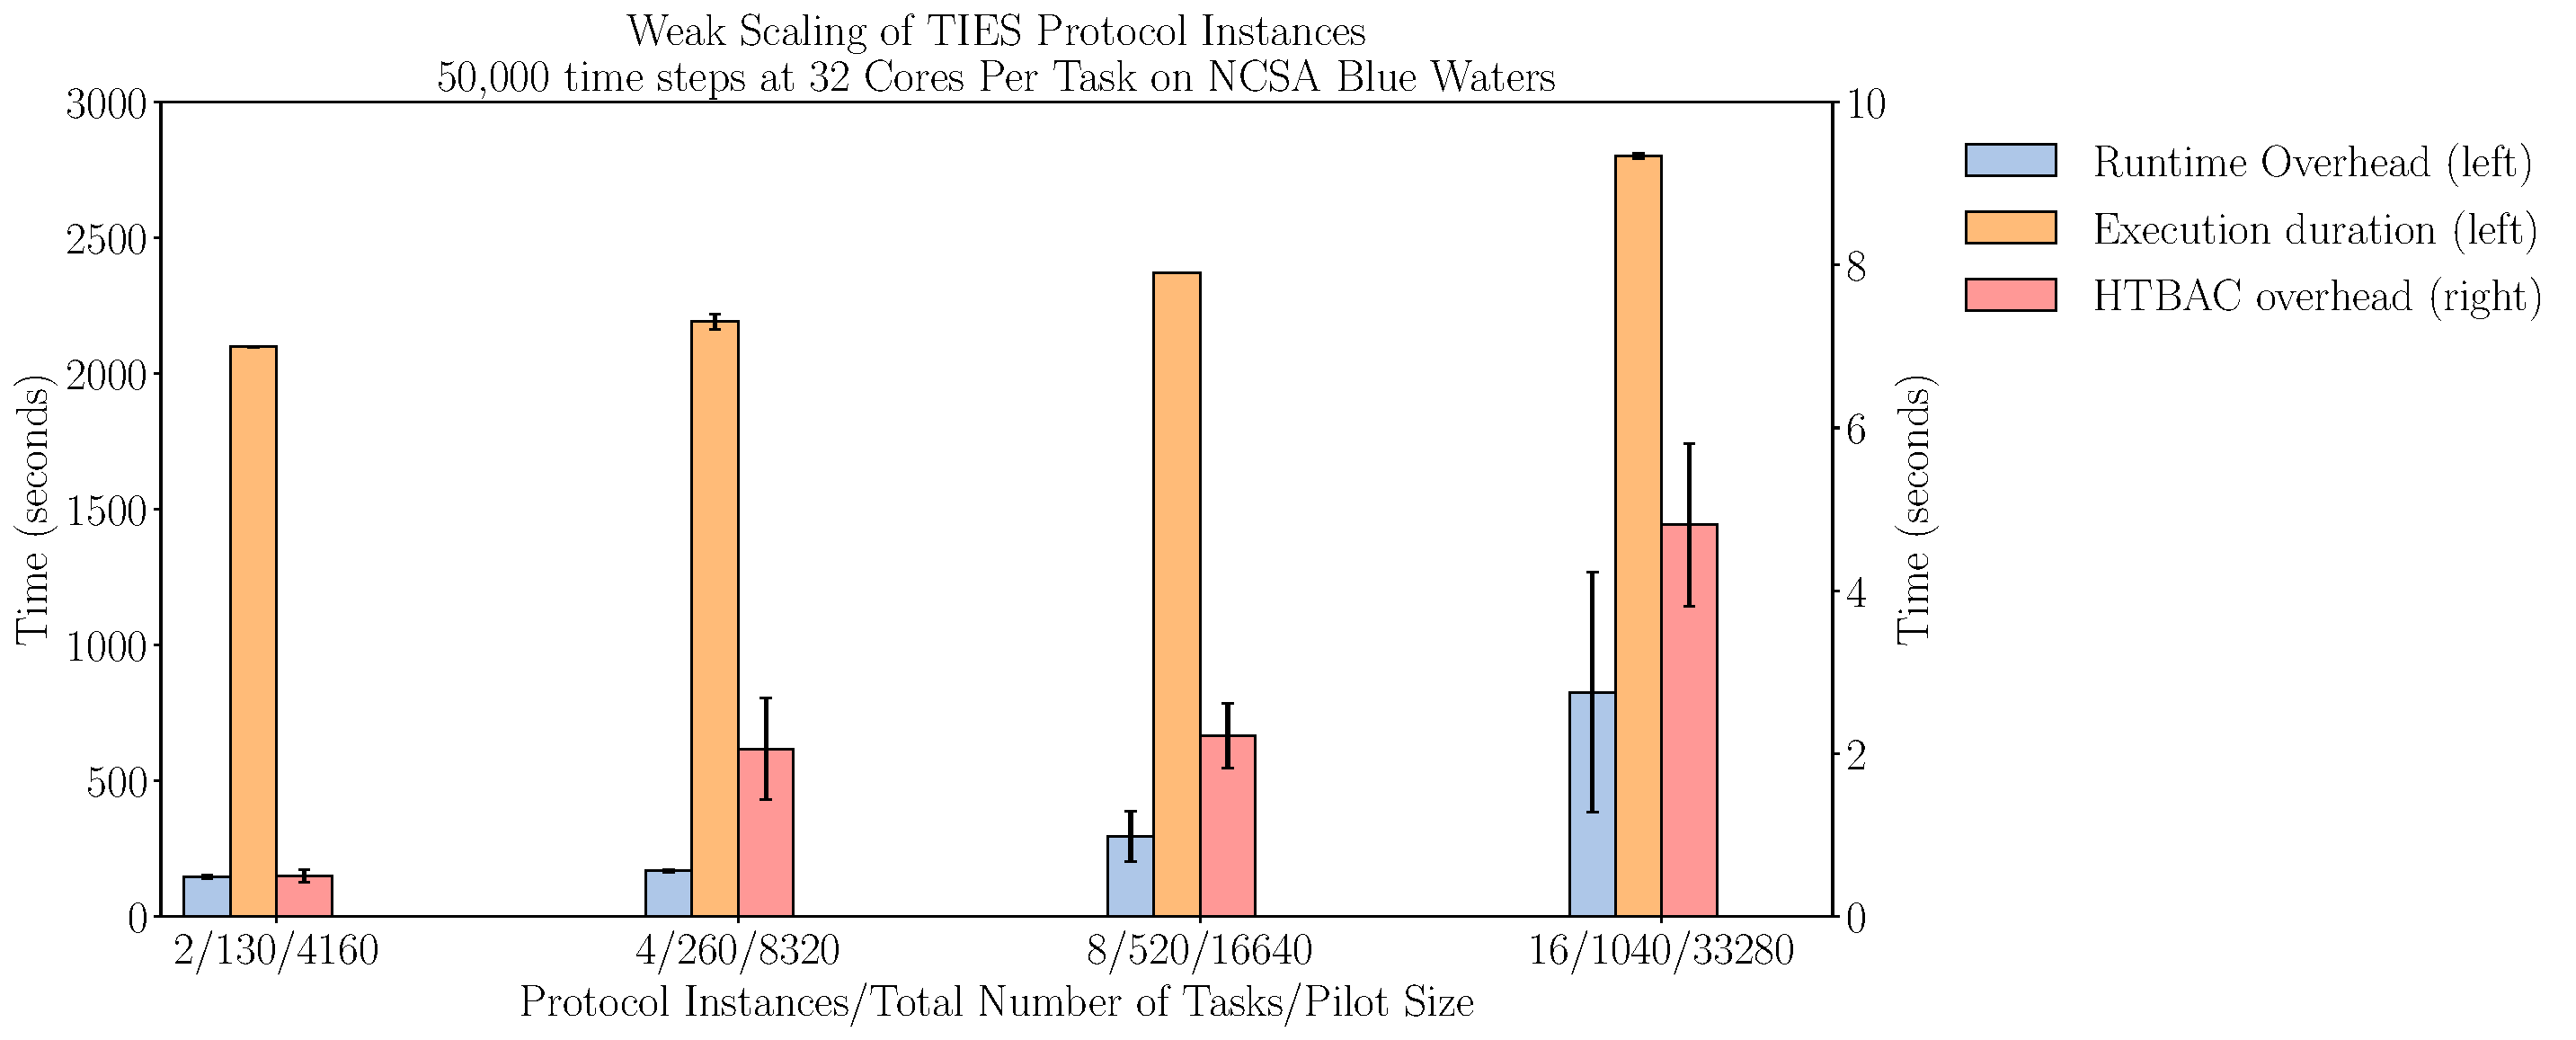
\includegraphics[width=\columnwidth]
   {weak_scaling_TIES_instances_50,000_timesteps_with_16_instances.pdf}
  \caption{Weak scaling properties of HTBAC. We investigate the
  weak scaling of HTBAC as the ratio of the number of protocol instances to
  resources is kept constant. Overheads of HTBAC framework (right), and RCT overhead 
  (left) and total execution time \(TTX\) (left) for experimental configurations investigating the 
  weak scaling of TIES. We ran two trials for each protocol instance 
  configuration. Error bars in \(TTX\) in 2 and 8-protocol runs are 
  insignificant.}
\label{fig:weak_scaling}
\end{figure}

Both ESMACS and TIES have been successfully used to predict binding affinities
quickly and accurately. 
In their standard non-adaptive forms TIES is approximately 2.5 times more expensive
than ESMACS.
The ligands investigated here are closely related so it could be expected that the
greater accuracy of TIES would be required to differentiate them.
However, in a drug design scenario many drug candidates would need to be investigated
meaning that optimizing the execution time while retaining (or improving) accuracy is
desirable. 
Given the very large number of drug candidates, it is imperative to
gain maximum insight into potential candidate compounds using time and
resources efficiently. 
This provides one clear motivation for the use of
adaptive methods which minimize the compute time used whilst producing binding
free energy estimates meeting pre-defined quality criteria (such as
convergence or statistical uncertainty below a given threshold).


Typically, datasets will involve ligands with a wide range of chemical 
properties which can impact not only the time to convergence, but the type 
of sampling required to gain accurate results.
In general, there is no way to know before running
calculations exactly which setup of calculation is required for a particular
system. 
Even within closely related ligands, such as the THQ based BRD4 ligands 
studied here, the $\partial U/\partial\lambda$ curve$\lambda$ integrated in TIES 
varies between physical systems (drugs). 
Consequently, the number (or the exact location) of the
$\lambda$ windows that will most impact the calculation are not known
\textit{a priori}, and change between systems. 
As multiple
simulations must be run for each window, sampling with a very high frequency
is expensive and impractical. Furthermore, adaptive placement of $\lambda$
windows is likely to better capture the shape of the
$\partial U/\partial\lambda$ curve, leading to more accurate and precise
results for a given computational cost (see figure~\ref{fig:adaptive}).

\begin{figure}[h!]
  \centering
  \begin{tikzpicture}
  \begin{axis} [scale=0.3, xmin=0, xmax=1, yticklabels={,,}, xtick={0, 1}]
  \addplot+[name path=true, mark=none, smooth, color=black] table {dg-tot-scaled.dat};

  \addplot[name path=approx_1, mark=o] coordinates {(0.00, 0.37126) (0.50, -51.44248) (1.00, -51.30041)};

  \addplot fill between[
    of = true and approx_1,
    split,
    every even segment/.style = {pattern color=red!50, pattern=north west lines},
    every odd segment/.style = {pattern color=red!50, pattern=north west lines},
    soft clip={domain=0:1},
  ];

  \end{axis}
  \end{tikzpicture}%
  \begin{tikzpicture}
  \begin{axis} [scale=0.3, xmin=0, xmax=1, yticklabels={,,}, xtick={0, 1}]
  \addplot+[name path=true, mark=none, smooth, color=black] table {dg-tot-scaled.dat};

  \addplot[name path=approx_1, mark=o] coordinates {
  (0.00, 0.37126)
  (0.20, -1.01429)
  (0.50, -51.44248)
  (0.80, -53.15965)
  (1.00, -51.30041)};

  \addplot fill between[
    of = true and approx_1,
    split,
    every even segment/.style = {pattern color=red!50, pattern=north west lines},
    every odd segment/.style = {pattern color=red!50, pattern=north west lines},
    soft clip={domain=0:1},
  ];

  \end{axis}
  \end{tikzpicture}%
  \begin{tikzpicture}
  \begin{axis} [scale=0.3, xmin=0, xmax=1, yticklabels={,,}, xtick={0, 1}]
  \addplot+[name path=true, mark=none, smooth, color=black] table {dg-tot-scaled.dat};

  \addplot[name path=approx_1, mark=o] coordinates {
  (0.00, 0.37126)
  (0.20, -1.01429)
  (0.30, 1.977340)
  (0.40, 4.27343)
  (0.50, -51.44248)
  (0.60, -55.19837)
  (0.80, -53.15965)
  (1.00, -51.30041)};

  \addplot fill between[
    of = true and approx_1,
    split,
    every even segment/.style = {pattern color=red!50, pattern=north west lines},
    every odd segment/.style = {pattern color=red!50, pattern=north west lines},
    soft clip={domain=0:1},
  ];

  \end{axis}
  \end{tikzpicture}

  \caption{Adaptive quadrature of the function $f(\lambda) = \partial U(\lambda)/\partial \lambda$ in the interval $[0, 1]$ using the trapezoidal rule. The figures from left to right show successive levels of recursion or bisection of the interval. The interpolation error is the difference (shaded area) between the interpolant and the actual function. If the error in an interval is too large, the interval is bisected.}
  \label{fig:adaptive}
\end{figure}


In order to support such
investigations, in addition to being scalable, HTBAC is enhanced to
support flexible resource reallocations schemes where resources can be moved
between simulations run using different protocols or systems, for example,
when one calculation has converged whilst another has not. This adaptability
makes it easier to manage complex programs where efficient use of resources
is required in order to achieve a time to completion of studies comparable to
those of high throughput chemistry.

The novel contributions of HTBAC are: (i) Unprecedented throughput: it allows
the concurrent screening for drug binding affinities of multiple compounds at
unprecedented scales, both in the number of candidates and resources utilized;
(ii) Agile selection of different binding affinity protocols: HTBAC supports
inter-protocol adaptivity, leading to resources being assigned at runtime to
the ``optimal" protocol (as determined by accuracy for given computational
cost); (iii) Support for intra-protocol adaptivity, which provides the
efficient execution of individual protocols.



% While RCT supports concurrent task execution up to 000 tasks on Blue Waters,
% the user is required to translate and codify each of these protocols with the
% corresponding mutation using the EnTK API, and scale these protocols
% based on the desired number of mutations and replicas [9]. We leverage
% the advanced resource management capabilities of RADICAL Cybertools and
% automate this process by providing a native selection of protocols where
% the user only provides the configuration files for each mutation, the number
% of replicas per mutation and the number of cores needed to support each
% protocol. To this effect, the framework uses EnTK to provide a higher level of
% abstraction that allows the user to interface closer to the science problem.

\subsection{Performance Metrics}\label{sec:performance}

% \subsection{Ensemble Molecular Dynamics}\label{sec:emd}

TIES is rigorous but computationally expensive and has a limited range of
applicability; ESMACS is approximate but can be employed across any set of
ligands at lower computational cost. Both protocols are designed to simulate a
large range of mutations. A single protocol instance represents a unique
physical system. Each protocol instance contains a pipeline which maps to a
sequence of simulations steps which include minimization, equilibration and
production MD simulation. These simulation pipelines are replicated, where
replicas differ only by their parameter configurations, namely initial
velocities, which are randomly generated and assigned by the MD engine at the
start of execution. ESMACS consists of 25 replicas i.e. 25 pipelines, while
TIES consists of 13 $\lambda$ windows, which are additional sampling
parameters, and 5 replicas for a total of 65 pipelines. The additional
pipelines in TIES contribute to the greater computational cost. Both protocols
run for a total of 6 ns simulation durations. ESMACS produces 3.5 GB/system
(24 MB/ns) while TIES produces 10 GB/system (24 MB/ns). Each simulation step
in TIES and ESMACS requires 32 cores. Protocols run approximately 10-12 hours,
depending on the physical system and the number of timesteps provided by the
user.

There are several measures of performance that are relevant. The most
pertinent is the weak scaling property which demonstrates the ability of HTBAC
to solve large number of drug candidates in essentially the same amount of
time (as the resources increase). To this effect, we investigated weak scaling
behavior for screening sixteen drug candidates concurrently using thousands of
multi-stage pipelines on more than 32,000 cores on NCSA Blue Waters (as shown
in Figure 2). Similar scaling has been demonstrated on other platforms such as
Titan for different protocols.


% ---------------------------------------------------------------------------
% Section VI
% ---------------------------------------------------------------------------
\section{Impact of Solution}\label{sec:impact}


The flexibility provided by HTBAC to run adaptive workflows offers huge advantages scientifically.
First, the intra-protocol adaptivity allows the automated optimization of calculations to ensure that
results are obtained with known precision across systems which may exhibit very different behavior (for example levels of `roughness' in the $\partial U/\partial\lambda$ curve in TIES).
This has a significant impact of the reliability of comparisons between runs.
The ability to switch between protocols on the other hand offers a mechanism through which `cheaper' approximate methods (such as ESMACS) can be used to scan large regions of chemical space, whilst more accurate and `expensive' ones are employed to investigate areas of specific interest (TIES).
This maps directly onto processes such as hit to lead optimization in drug discovery and cold be of particular use in investigating activity cliffs.
This is a phenomena where small chemical changes provide large differences in drug efficacy.
If changes are detected using an approximate method it is important to verify that they come from
real chemical effects and not simply inaccuracies in the computational algorithm employed.

The scale enabled by HTBAC also has an impact on the potential for scientific discovery using free energy calculations.
Most studies in the literature are limited to the investigation of tens of protein-ligand complexes.
In order to establish the validity of particular combinations of forcefield and simulation protocol and
quantify uncertainties much larger campaigns are needed.
Our ensemble has already provided evidence that the variability in single runs is sufficient to
swamp true differences between systems of interest.
The combined need for both large numbers of systems and multiple repeats of each one produces a requirement
for middleware to manage huge numbers of simulations.

HTBAC allows the concurrent screening
for drug binding affinities of multiple compounds at unprecedented scales,
both in the number of candidates and resources utilized. Specifically, we
investigated weak scaling behavior for screening sixteen drug candidates
concurrently using thousands of multi-stage pipelines on more than 32,000
cores on NCSA Blue Waters. This permits a rapid time-to-solution that is
essentially invariant with respect to the calculation protocol,
size of target system and number of ensemble simulations. In addition,
HTBAC enabled the adaptive execution of the TIES protocol
providing greater convergence (i.e., lower errors) for a given amount of
computational resources.

These developments fit into a wider vision in which the use of
flexible and responsive computational protocols produce accurate,
precise and reproducible estimates of the free energy of binding with
meaningful error bars. Not only would this allow for wider uptake of
computational techniques in industrial settings but opens up possibilities
of using these technologies in clinical decision support scenarios. By creating
a `digital twin', where the target protein is based on the real patients
genetic sequence, a specific individuals response to different
treatments could be predicted.


% ---------------------------------------------------------------------------
% Section VII
% ---------------------------------------------------------------------------
\section{Analysis of Solution}\label{sec:analysis}

Our previous work deploying both ESMACS and TIES has typically involved 
comparing 10 to 20 computed binding affinities. In the original BRD4 inhibitor 
study, conducted in collaboration by UCL and GlaxoSmithKline \cite{Wan2017brd4}, 
16 drugs were investigated. All drugs were studied using ESMACS and 12 TIES 
transformations were performed. The non-adaptive protocols required 
approximately 10k and 25k core hours per system for ESMACS and TIES 
respectively, for a total of  $\sim$460k core hours for the whole study. Without 
HTBAC, each system was run by hand. This scale of study is only appropriate for 
retrospective analysis showing the potential of the methods involved. For 
\textit{in silico} approaches to have a real impact in industrial scenarios much 
larger numbers of systems must be run, which is not practical without 
appropriate middleware. HTBAC satisfies this need by providing a logically 
programmable interface which facilitates the routine of running studies 
requiring sustained usage of millions of core hours per day.

The drug design process involved the filtering of millions of compounds to 
smaller number of 'hits' that bind the target protein and then further 
refinement to 'leads' that form the basis of candidate drugs. Encapsulation of 
the ESMACS and TIES protocols in HTBAC means that these protocols can be 
efficiently applied to the middle and end of this process. Adaptive 
functionality means that HTBAC can ensure efficient use of the resources 
depending on the properties of the ligands under investigation. This flexibility 
also provides a platform to run the varied simulation campaigns needed to stress 
test protocols and forcefields in order to further refine our modeling approaches.


% ---------------------------------------------------------------------------
% Demonstration
% ---------------------------------------------------------------------------
\section{Impact and Result}\label{sec:demo}

% If invited to the final round of SCALE 2018, we will demonstrate the following:

% \begin{enumerate}

% \item The number of drug candidates screened as a function of the number of cores 
% marshaled; equivalently as a function of the number of core-hours consumed.

% \item Demonstration of switching between protocols so as to achieve "optimal"
% configurations so that best estimates for binding affinities for a given amount
% of resources. Traces of execution that will display adaptivity and resource
% allocation across protocols.

% \item Additional measures of performance and scale

% \item How scalable, accurate and rapid binding affinity calculation using
% HTBAC can enable effective clinical decision making


% \end{enumerate}

We demonstrate how scalable, accurate and rapid binding affinity calculation 
using HTBAC can enable effective clinical decision making by showing performance 
and scale of the number of drug candidates screened as a function of the 
number of core-hours. In addition, we show additional functionality of HTBAC 
to enable the adaptive execution of the TIES protocol, thereby providing greater 
convergence (i.e., lower errors) for a given amount of computational resources. 
As such, HTBAC advances binding affinity calculation to support scale and 
optimize for time-to-insight for investigative drug screening computational 
campaigns. 


% ---------------------------------------------------------------------------
% BIBLIOGRAPHY
% ---------------------------------------------------------------------------
\bibliographystyle{unsrt}
\bibliography{rutgers,ucl,mskcc}

\end{document}
